\documentclass[12pt, oneside]{article}
\usepackage[letterpaper, margin=1in, headsep=0.5in]{geometry}
\usepackage[english]{babel}
\usepackage[utf8]{inputenc}
\usepackage{amsmath}
\usepackage{amsfonts}
\usepackage{amssymb}
\usepackage{tikz}
\usetikzlibrary{quotes, angles}
\usepackage{graphicx}
%\usepackage{pgfplots}
%\pgfplotsset{width=10cm,compat=1.9}
%\usepgfplotslibrary{statistics}
%\usepackage{pgfplotstable}
%\usepackage{tkz-fct}
%\usepackage{venndiagram}

\usepackage{fancyhdr}
\pagestyle{fancy}
\fancyhf{}
\rhead{\thepage \\Name: \hspace{1.5in}.\\}
\lhead{BECA / Dr. Huson / 10.3 Geometry\\* Algebra review}

\renewcommand{\headrulewidth}{0pt}

\begin{document}
Solve each problem. Use $x$ as the variable. Show the check.
  \begin{enumerate}
\subsubsection*{Word Problem Wednesday}

  \item A DJ charges \$225 to play for a party plus \$80 per hour. The total for one event was \$625.
  \begin{enumerate}
    \item What would this problem ask you to solve for? \\[0.5cm]
    \hspace{1cm} $x=$ the number of $\rule{3cm}{0.15mm}$
    \item Make a table of $x$ and the cost. Start with $x=0$ \\[0.5cm]
    \begin{center}
      \begin{tabular}{|c|r|}
      \hline
      $x$ & cost\\
      \hline
      0 &  \\
      \hline
      1 &  \\
      \hline
      2 &  \\
      \hline
      3 &  \\
      \hline
      4 &  \\
      \hline
      5 &  \\
      \hline
      6 &  \\
      \hline
      \end{tabular}
    \end{center}
    Show the row differences. Circle the row in the table with the right cost.
    \item Write an equation for the problem of the form $y=mx+b$, and solve it for $x$ \vspace{3.5cm}
    \item Check the answer \vspace{2.5cm}
    \item Spicy: How much would be the tax at 11\% on the total charge?
  \end{enumerate}

\newpage
For each problem, use $x$ as the variable, make a table, write an equation, solve it, and show the check. \\%[0.5cm]

  \item Debbie has collected two dozen plastic bottles to recycle. She plans to collect an additional 24 bottles each week. Her goal is to collect a total of 120. \vspace{8cm}

  \item A plane rental service charges a \$1500 deposit and \$300 per hour to rent a small aircraft. Alex has budgeted \$3000 to spend on a day trip.

\newpage
  \item The entrance fee at Six Flags is \$17.50 and each ride costs \$1.50. Elizabeth has \$35. \vspace{8cm}

  \item A basketball free throw video game gives you a starting score of 100 points, and you lose 2 points with each miss. Ishmael wants to stop when he reaches 24 points.

\newpage
  \item There are two cable TV plans. Disney has a start-up fee of \$75 and costs \$25 per month. The HBO plan costs \$5 to start, but charge \$40 per month. After how many months will they cost the same?  \vspace{8cm}

  \item Dr. O'Grady's Swedish ivy plant is $2 \frac{1}{2}$ inches tall and grows one-half inch per week. His poison ivy cutting is 1 inch long and grows $\frac{3}{4}$ inches per week. After how many weeks will the poison ivy be the longer plant?

\newpage
\subsubsection*{Graphing linear functions}
Use pencil for graphs. Mark at least some of the values on each axis. Label each function with its name or equation.
\item Two sisters play a card game to win points. Juliana wins 2 points in each hand, while her little sister only wins 1 point per hand. To be fair, Juliana gives her sister 3 points to begin with as a handicap. \\
The game is to seven points.
  \begin{enumerate}
      \item Make a table showing how many points each sister has with each hand played. \bigskip
      \item Write down the slope of both sister's scores based on the differences. \bigskip
      \item Draw a line on the graph representing the score of each sister.
      \item Label the intersection $T$ for ``tied."
      \item On the $x$-axis mark 7 as the end of the game.
      \item Who wins? \bigskip
  \end{enumerate}

  \begin{center} %4 quadrant regents grid
  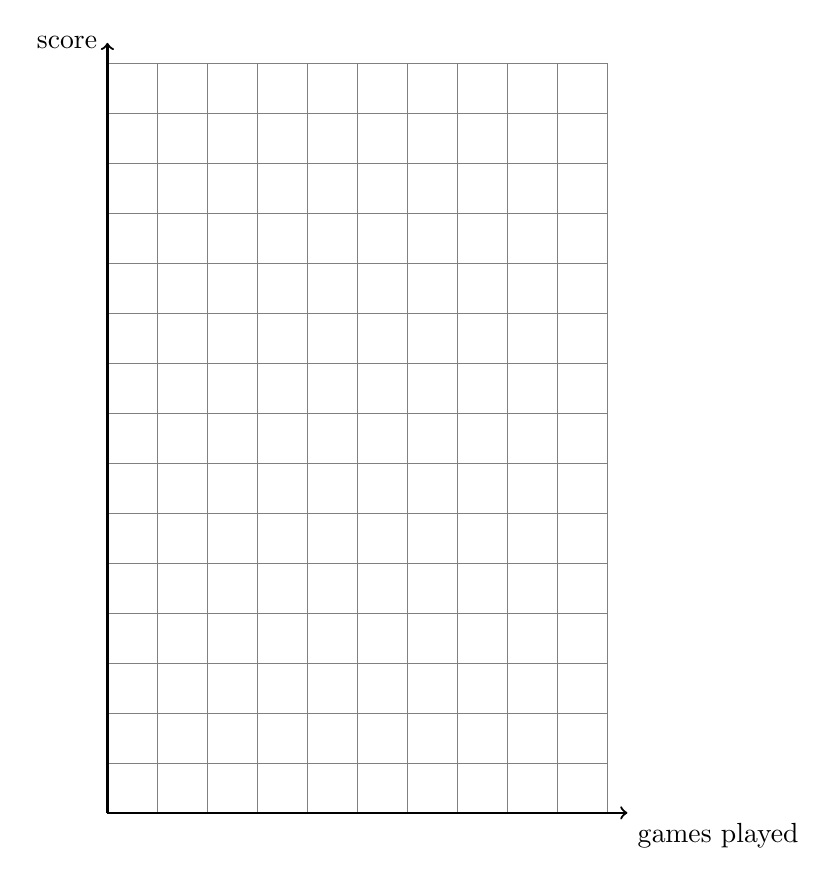
\begin{tikzpicture}[scale=0.635]
    \draw [help lines] (0,0) grid (10,15);
    \draw [thick, ->] (0,0) -- (10.4,0) node [below right] {games played};
    \draw [thick, ->] (0,0)--(0,15.4) node [left] {score};
  \end{tikzpicture}
  \end{center}


\newpage
  \item $4x^2+3x -7 -2x^2-x+4$ \vspace{3cm}
  \item $3(a^2-2a +1) -2(a^2-a-4)$ \vspace{3cm}

\subsubsection*{Solve equations}

Solve for the value of $x$.
\item   $10=x-3x$ \vspace{3cm}
\item   $\frac{1}{2}(6-2x)=4x$ \vspace{3cm}
\item   $11=\frac{1}{3}x+2x-10$ \vspace{3cm}


\subsubsection*{Slope-intercept form}

What is the slope and $y$-intercept of each equation?
\item   $y=2x-3$ \vspace{2cm}
\item   $4x+2y=6$ \vspace{3cm}


\subsubsection*{Function substitution}
\item Given $f(x)=4x+7$. Simplify $f(2)$. \vspace{4cm}
\item Given $\displaystyle f(x)=-\frac{(12+4x)}{11}$. Simplify $f(-3)$.

\newpage

\item
  \begin{enumerate}
    \item Mark and label the point $P(4, 5)$ on the graph below.
    \item The line $L_1$ has a $y$-intercept of 3 and passes through point $P$. Graph $L_1$.
    \item What is the slope of line $L_1$? \vspace{2cm}
    \item What is the equation of line $L_1$? \vspace{2cm}
    \item A second line, $L_2$ has the equation $3x+4y=-8$. Plot $L_2$ on the graph.
    \item On the graph, mark the intersection of the two lines, $Q$, as an ordered pair.
  \end{enumerate}

  \begin{center} %4 quadrant regents grid
    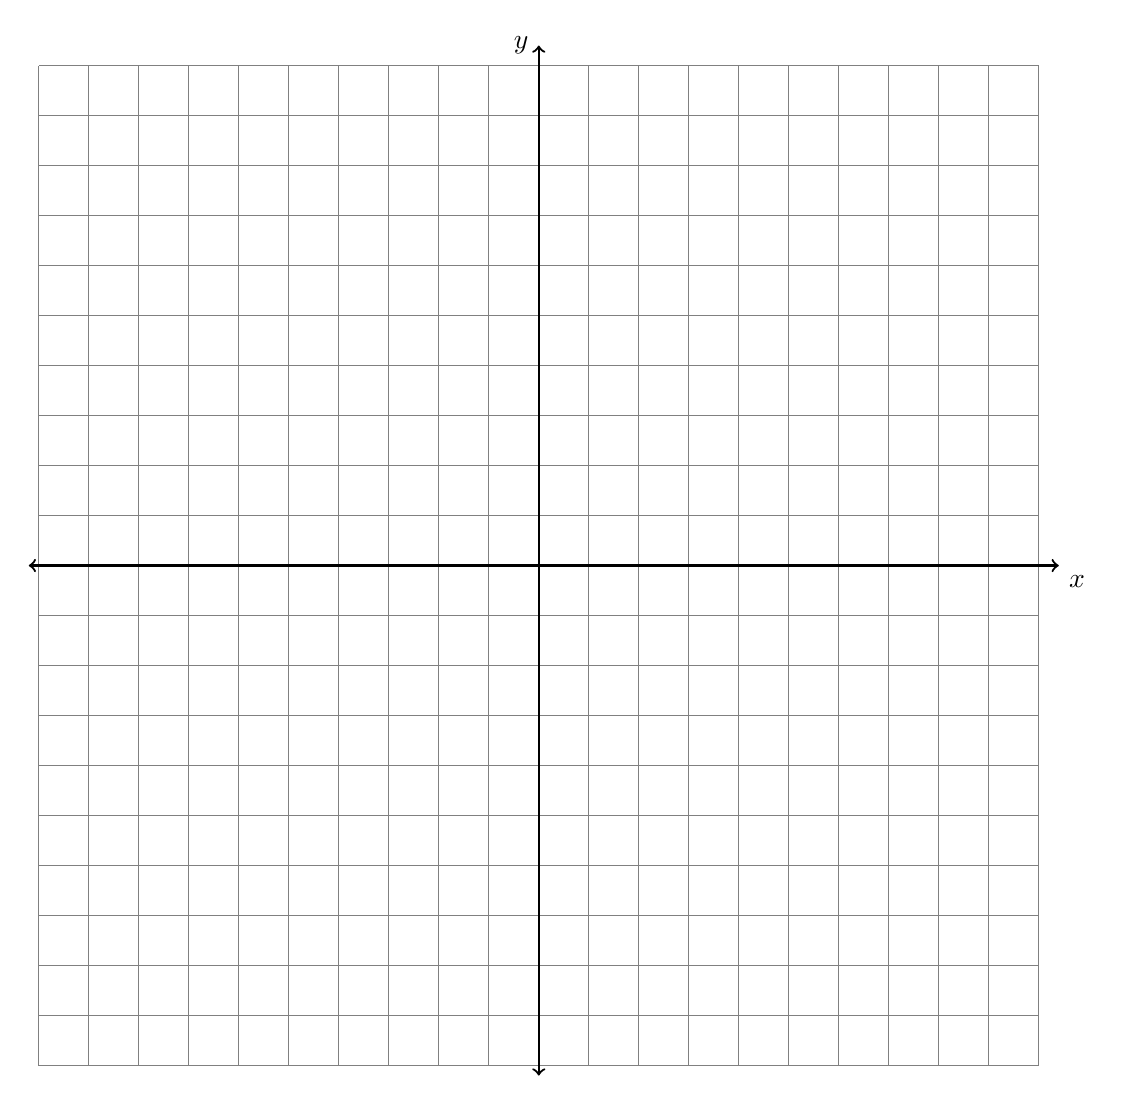
\begin{tikzpicture}[scale=0.635]
      \draw [help lines] (-10,-10) grid (10,10);
      \draw [thick, <->] (-10.2,0) -- (10.4,0) node [below right] {$x$};
      \draw [thick, <->] (0,-10.2)--(0,10.4) node [left] {$y$};
    \end{tikzpicture}
  \end{center}

\newpage
  \item Solve the system of equations by graphing each line and marking the intersection as an ordered pair.
    \[x+y=7\]
    \[y=3x+3\]

\begin{center} %4 quadrant regents grid
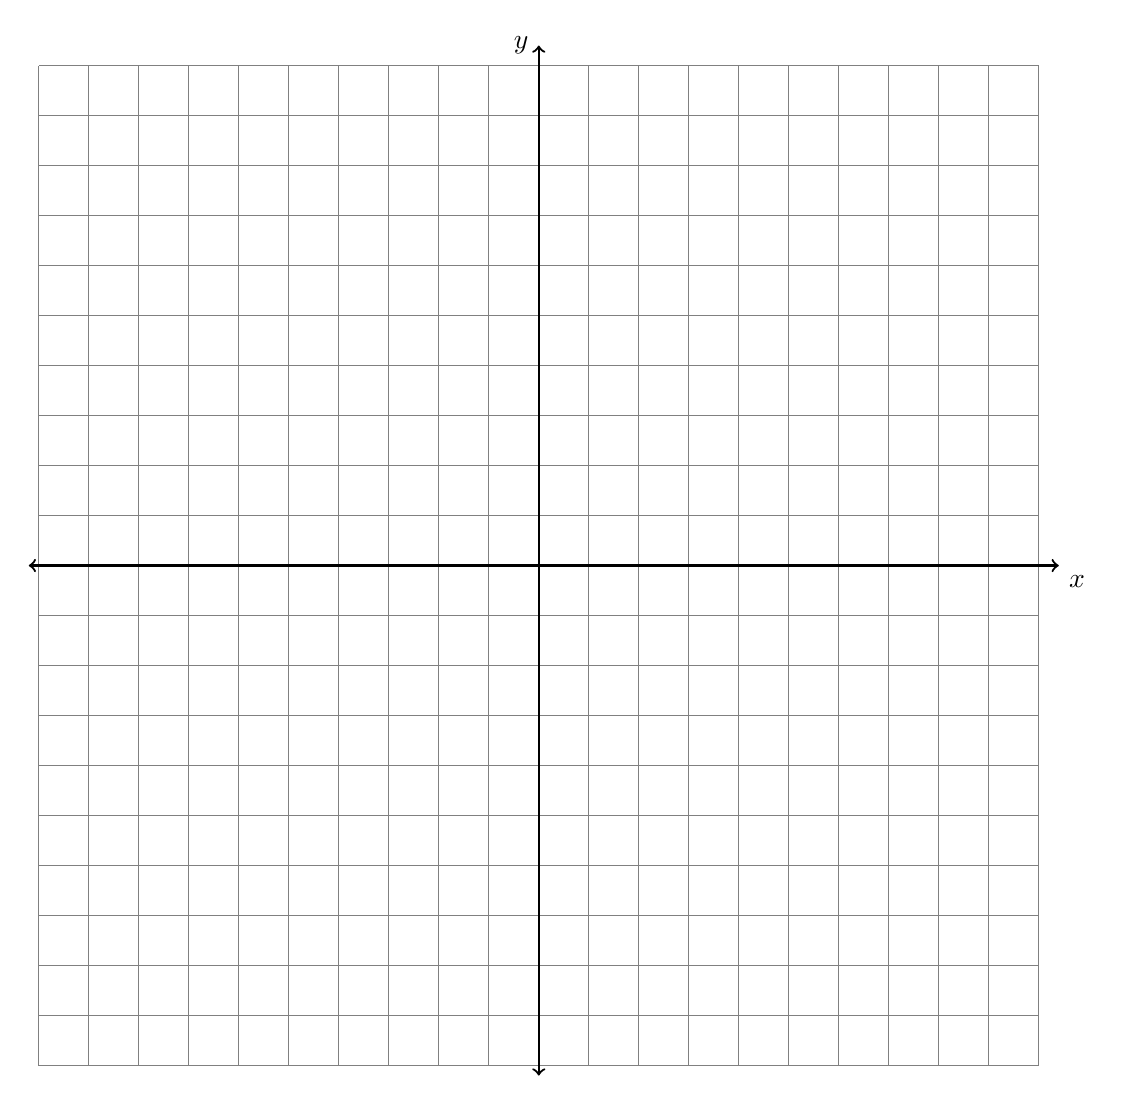
\begin{tikzpicture}[scale=0.635]
  \draw [help lines] (-10,-10) grid (10,10);
  \draw [thick, <->] (-10.2,0) -- (10.4,0) node [below right] {$x$};
  \draw [thick, <->] (0,-10.2)--(0,10.4) node [left] {$y$};
\end{tikzpicture}
\end{center}

\newpage
  Solve each system algebraically.
  \item
  $2x-4y=14$\\*
  $5x+4y=7$ \vspace{6cm}

  \item
  $2x-y=-7$\\*
  $3x+4y=17$  \vspace{6cm}


  \item Is the expression $2-\sqrt{5}$ rational, irrational, or neither? Explain.

\newpage
  \item Oceanside Bike Rental Shop charges a 17 dollar bike fee plus 6 dollars an hour for renting a bike. Jeffrey paid 53 dollars total. How many hours did he pay to have the bike checked out? \vspace{6cm}

  \item Three friends go bowling. The cost per person per game is \$5.30. The cost to rent shoes is \$2.50 per person. Their total cost is \$55.20. How many games did they play? \vspace{6cm}

  \item The admission fee at a small fair is \$1.50 for children and \$4.00 for adults. On a certain day, 40 people enter the fair and \$85.00 is collected. How many children and how many adults attended?

\newpage
\subsubsection*{Parallel and perpendicular linear equations}

  \item What is the equation of the line with a slope of 2 passing through the point $(0,1)$? \vspace{4cm}
  \item What is the equation of a line parallel to $y=-2x+1$ with a $y$-intercept of 4? \vspace{4cm}
  \item What is the slope of a line perpendicular to the line $x-2y=16$? \vspace{4cm}

\end{enumerate}
\end{document}
